\section{Background \& Experiment Setup}
\label{sec:background}

We provide a brief background on video conferencing transport, technology, and
architecture \rev{before turning to}{followed by a description of} our experiment setup.

\subsection{Video Conferencing Applications}

Most modern VCAs use Real-time Transport Protocol (RTP)~\cite{schulzrinne1996rtp, schulzrinne2003rfc3550} or its variants~\cite{baugher2004secure, zoom_rtp} to
transmit media content. The audio and video data is generally transmitted over
separate RTP connections. RTP also uses two other protocols in conjunction,
Session Initiation Protocol (SIP)~\cite{rosenberg2002sip} to establish
connection between clients and RTP Control Protocol
(RTCP)~\cite{schulzrinne2003rfc3550} to share performance statistics and
control information during a call. Despite using well-known protocols, VCAs
can differ from each other significantly across the following dimensions:


\begin{itemize}
    \itemsep=-1pt
    \item \textbf{Network mechanisms}: RTP and \rev{the} associated protocols are
        implemented in the application-layer. Thus, the specific
        implementation of the protocols can vary across VCAs. For instance,
        Zoom reportedly uses a custom extension of RTP~\cite{zoom_rtp}).
        Furthermore, the key \rev{network}{transport-layer} functions, i.e., congestion control and
        error recovery, can also be different and proprietary. 

    \item \textbf{Application-layer parameters}: These include media encoding
        standards and default bitrates. More recent video codecs (e.g., VP9,
        H.264) can encode at the same video quality with fewer bytes when
        compared to older codec (e.g., VP8), albeit with a higher compute
        overhead~\cite{bienik2016performance}. 
    
    \item \textbf{Streaming architecture}: VCAs can either choose to use
        direct connections or use relay servers. Centralized servers are
        almost always used for multi-point calls to combine data from multiple
        users. VCAs can differ in the exact strategies of data combination as
        well as the geographic footprint of their servers. For instance, Zoom
        rapidly expanded its server infrastructure to support increased call
        volume because of COVID-19~\cite{liu2020characterizing}. 

\end{itemize}
\noindent
Differences across one or more of these factors can lead to different VCA
network utilization and performance. In this paper, we aim to dig deeper into
some of these differences for a subset of VCAs. 


\subsection{Experiment Setup} 
\label{subsec:setup}

\paragraph{Video Conferencing Applications}:
In this paper, we study three popular VCAs---\zoom, Google \meet, and Microsoft \teams.
These VCAs have been used extensively worldwide over the past year, especially
in enterprises and educational institutions~\cite{vca_share}.  Teams and Zoom
provide desktop applications as well as browser clients, whereas Meet is ``native"
in \rev{the}{} Chrome. Most of our tests are conducted using the desktop
applications for Teams and Zoom, and using the Google Chrome browser for Meet.
In-browser tests for Teams and Zoom are specified by \textit{\teamsbrowser}
and \textit{\zoombrowser}, respectively. We use Chrome (Meet) version
89.0.4389, Zoom client version 5.6.1, and Teams client version 1.4.00.7556. 
\rev{}{Note that we use the enterprise versions of all three VCAs
provided by our University accounts. Moreover, the associated Zoom account used for the experiments had HD enabled, while default settings are used for Meet and Teams. }

\paragraph{Laboratory Environment}:
We conduct experiments in a controlled environment.  We begin by describing our experimental setup for a 2-party call. We use two identical laptops, referred to as V1 and V2, representing the two VCA clients. Each laptop is a Dell Latitude 3300 with a screen resolution of 1366 $\times$
768 pixels and running Ubuntu 20.04.1. The laptops have a wired connection to
a Turris Omnia 2020 router and access a dedicated 1~Gbps symmetric link
to the Internet.  Each experiment consists of a call between V1 and V2 under a
pre-specified network bandwidth profile and VCA. \rev{The bandwidth profile is
emulated by shaping the link between V1 and the router using traffic control
(\texttt{tc}).}{
Traffic Control (\texttt{tc}), specifically the hierarchical token bucket queuing discipline, is used at the router to emulate the bandwidth profile.}  
A pre-recorded talking-head video\footnote{It would be inappropriate to use the 
device webcam as the video, because without movement, VCAs compress the video and ultimately send at a much lower rate than during a normal call.} with a resolution of 1280 $\times$ 720 is used as the video source for the call, using \texttt{ffmpeg}.
This is done to both replicate a real video call and ensure consistency across
experiments. All experiments are conducted with the laptop lid open and the application window maximized. 

\rev{}{In all cases, the 
participants join calls that are initiated in real-time by one of the participants. For two-person calls, this means one participant launches the meeting and the 
other joins shortly thereafter. Such ad-hoc calls may be different from scheduled calls wherein VCAs can perform few optimizations including pre-allocation of relay servers. 
While choice of relay servers can significantly impact end-user experience, especially for geographically distributed clients~\cite{jiang}, we believe the
paths to the relay servers are likely not the bottleneck in our case for two reasons: i) all of our participants are located within the University network with well-provisioned access link and upstream transit connections, and ii) the experiments are conducted in Chicago, which is a major population region. It is likely that Teams, Meet, and Zoom have nearby relay servers to provide good service.}


\begin{figure*}[t!]
\begin{subfigure}[t]{0.33\textwidth}
    \centering
    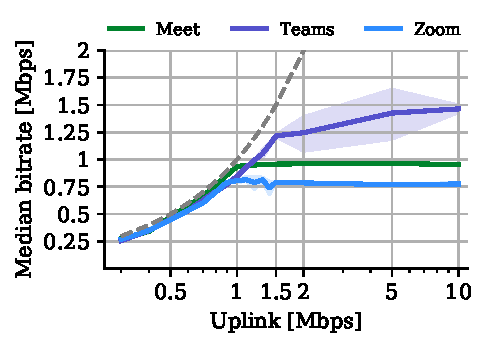
\includegraphics[width=\textwidth,keepaspectratio]{figures/static/uplink.pdf}
    \caption{Uplink bandwidth vs network bitrate %\jamie{label $x = y$}
    }
	\label{subfig:uplink_bitrate}
\end{subfigure}\hfill
\begin{subfigure}[t]{0.33\textwidth}
\centering
    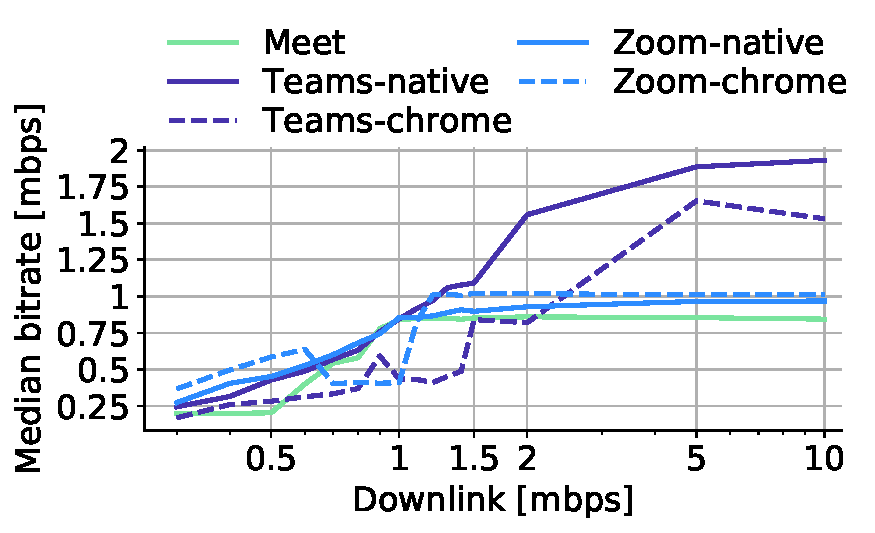
\includegraphics[width=\textwidth,keepaspectratio]{figures/static/downlink.pdf}
    \caption{Downlink bandwidth vs network bitrate}
	\label{subfig:downlink_bitrate}
\end{subfigure} \hfill
\begin{subfigure}[t]{0.33\textwidth}
\centering
    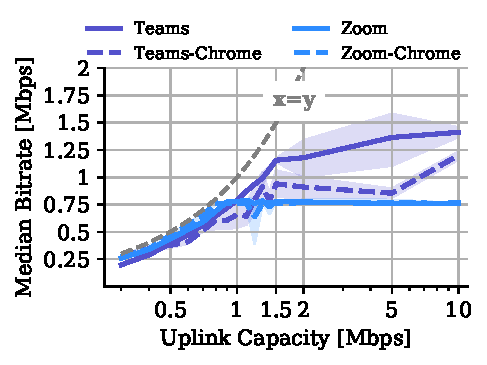
\includegraphics[width=\textwidth,keepaspectratio]{figures/static/uplink_browser.pdf}
    \caption{Impact of VCA platform %\jamie{capitalize Chrome}
    }
	\label{subfig:uplink_browser}
\end{subfigure} 
\vspace{-1em}
\caption{Network utilization under different shaping levels. The bands represent 90\% confidence intervals.}
\label{fig:static}
\end{figure*}
%on the laptop and router for uplink and downlink shaping, respectively. During the competition experiments, all shaping occurs at the router.

\paragraph{Automating Experiments}: To conduct experiments at scale, we
automated the entire call process. We take several steps to enable automated calls.  We use the Python PyAutoGUI package~\cite{pyautogui} to
automate joining and leaving calls. The package \rev{enables}{allows us} to programmatically
control the keyboard and the mouse by specifying coordinates or visual
elements on the screen. For \zoombrowser, we encountered CAPTCHA before
joining a call on the default browser. Using the Selenium-based Chrome
browser~\cite{selenium}, however, enabled us to bypass the CAPTCHA. Note \rev{}{that} the
experiments using Selenium are run exactly as \rev{it}{they} would be in default Chrome
browser. The workflow is controlled from V1, with TCP sockets used to
coordinate between V1 and V2.  We modify this setup slightly for subsequent
experiments (e.g., multi-party calls); those slight modifications are
described in the respective sections.


%%%%%%%%%%%%%%%%%



\begin{comment}
\paragraph{Performance metrics}: We mainly focus on the following application metrics. 
\begin{itemize}
    \item \textbf{Network bitrate}
    \item Video resolution
    \item Frames per second
    \item Freeze count
    \item Freeze duration
    \item Jitter-buffer delay 
\end{itemize}

Most of our analysis is using network bitrate. We consider other application performance metrics when they can be extracted from Google Chrome\footnote{chrome://webrtc-internals}. Our analysis shows that there is a strong correlation between network bitrate and application performance. This is intuitive as real-time streaming is characterized by low latency and thus any network interruptions usually lead to degradation in application performance. 


\subsection{Measurement Method}
The measurement setup consists of several components:

Hardware
\begin{itemize}
    \item matched laptops for nominal flows
          \begin{itemize}
              \item All Linux; caveats -- may not be the most-maintained apps
              \item What laptops, for the many-laptop tests?
          \end{itemize}
    \item turris router for control of single shaped link
    \item private iperf server on university network
\end{itemize}

\begin{itemize}
    \item traffic control scripts
    \item autogui; selenium for browser
          \begin{itemize}
              \item Important that we have the screen up -- see e.g., the tweet, but maybe chase the paper, about the struggle of getting the machines to actually render flows being important.
              \item client vs browser
              \item sw versions?
          \end{itemize}
    \item pcap, iperf logs
    \item webrtc
          \begin{itemize}
              \item difference between meet and zoom 
          \end{itemize}
    \item Zoom API access (\& limitations?)
    \item control over sockets?
\end{itemize}

\begin{table*}[t!]
\centering
\begin{tabular}{|c|c|c|c|c|}
\hline
\paragraph{VCA} & \textbf{Platforms}     & \textbf{Encoding} & \textbf{Direct connection?} & \textbf{Network Protocol} \\ \hline
\hline 
Meet  & Browser, Phone         & VP9/VP8   & No                 & RTP (WebRTC)     \\ \hline
Teams & Native, Browser, Phone & VP9       & ?                  & RTP              \\ \hline
Zoom  & Native, Browser, Phone & H.264 SVC & Yes                & Variation of RTP \\ \hline
\end{tabular}
\caption{Design parameters of selected VCAs}
\label{tab:vca_overview}
\end{table*}
\end{comment}

